\RequirePackage{fix-cm}
\documentclass[fontsize=13pt,a4paper,oneside,DIV=calc,chapterprefix=true]{scrbook}

% ---- Gói hỗ trợ tiếng Việt và bảng mã ----
\usepackage[utf8]{vietnam}
\usepackage{amsmath,amssymb,amsfonts}
\usepackage{mathptmx}

% ---- Định dạng trang và căn lề ----
\usepackage{geometry}
\geometry{a4paper,top=2.2cm,bottom=2.2cm,left=2.8cm,right=2.2cm}
\usepackage{setspace}
\setstretch{1.3}

% ---- Đồ họa, màu sắc và hình vẽ TikZ ----
\usepackage{graphicx}
\usepackage{subcaption}
\usepackage{xcolor}
\usepackage{tikz}
\usetikzlibrary{arrows.meta, positioning, fit, backgrounds, calc, shapes.geometric}

% ---- Bảng biểu và danh sách ----
\usepackage{booktabs}
\usepackage{array}
\usepackage{multirow}
\usepackage{tabularx}
\usepackage{longtable}
\newcolumntype{P}[1]{>{\centering\arraybackslash}p{#1}}
\newcolumntype{M}[1]{>{\centering\arraybackslash}m{#1}}
\usepackage{enumitem}

% ---- Tiêu đề trang, liên kết và caption ----
\usepackage{fancyhdr}
\usepackage{float}
\usepackage{caption}
\usepackage{hyperref}
\hypersetup{
    colorlinks=true,
    linkcolor=blue,
    filecolor=magenta,
    urlcolor=cyan,
    citecolor=blue
}

\definecolor{blueborder}{RGB}{0,102,204}
\definecolor{eelanblue}{RGB}{220,235,252}
\definecolor{eelanorange}{RGB}{254,237,222}
\definecolor{eelangreen}{RGB}{229,245,224}
\definecolor{eelanpurple}{RGB}{242,234,250}

% Macro chèn ảnh an toàn: Nếu có ảnh thì hiển thị, nếu chưa có thì hiển thị khung placeholder
\newcommand{\safeimage}[3]{%
    \IfFileExists{#1}{%
        \includegraphics[#2]{#1}%
    }{%
        \fbox{%
            \begin{minipage}[c][4.5cm][c]{0.88\linewidth}
            \centering
            \footnotesize \textbf{[Ảnh minh họa kết quả thực nghiệm]}\\[0.15cm]
            Đường dẫn tệp: \texttt{\detokenize{#1}}\\[0.1cm]
            \textit{#3}
            \end{minipage}%
        }%
    }%
}

% Định nghĩa trang bìa tiêu chuẩn theo mẫu Trường ĐHKHTN - ĐHQGHN
\newcommand{\customtitlepage}{
\begin{titlepage}
\thispagestyle{empty}
\begin{center}
    \setlength{\fboxsep}{4pt}
    \setlength{\fboxrule}{1.2pt}
    {\color{blueborder}\fbox{\fbox{\color{black}
    \begin{minipage}{0.93\textwidth}
    \vspace{0.5cm}
    \begin{center}
        \textbf{\large ĐẠI HỌC QUỐC GIA HÀ NỘI}\\
        \textbf{\large TRƯỜNG ĐẠI HỌC KHOA HỌC TỰ NHIÊN}\\
        \textbf{\large KHOA TOÁN - CƠ - TIN HỌC}\\[0.6cm]

        \IfFileExists{logo/logo_hus.jpg}{%
            \includegraphics[width=3.2cm]{logo/logo_hus.jpg}\par
            \vspace{0.5cm}
        }{%
            \vspace*{1.5cm}
        }

        \textbf{{\LARGE MỘT SỐ VẤN ĐỀ CHỌN LỌC VỀ THỊ GIÁC MÁY TÍNH}}\\[0.2cm]
        % \textbf{\large MÃ HỌC PHẦN: MAT3563}\\[0.4cm]
        \hrule height 1.2pt
        \vspace{0.6cm}
        \textit{\Large BÁO CÁO MINI PROJECT 01}\\[0.35cm]
        \textbf{\huge PHÂN TÍCH KHỐI E-ELAN VÀ ỨNG DỤNG TRONG PHÂN LOẠI ẢNH, PHÁT HIỆN ĐỐI TƯỢNG}\\[0.4cm]
        \textbf{\Large (CATS, DOGS, PANDA)}\\[0.6cm]
        \hrule height 1.2pt
        \vspace{1.3cm}

        \begin{flushleft}
        \hspace{0.8cm}\textbf{\large Giảng viên hướng dẫn:} TS. Cao Văn Chung \\[0.4cm]

        \hspace{0.8cm}\textbf{\large Nhóm sinh viên thực hiện:}\\[0.25cm]
        \hspace{0.8cm}
        \begin{tabular}{@{}llll@{}}
            \textbf{STT} & \textbf{Họ và tên} & \textbf{MSSV} & \textbf{Lớp} \\[0.1cm]
            1 & Nguyễn Đức Quang & 23001918 & K68A4\\
            2 & Hà Minh Quang    & 23001916 & K68A4\\
        \end{tabular}
        \end{flushleft}

        \vfill
        {\large \textbf{Hà Nội, 10/2026}}
        \vspace{0.5cm}
    \end{center}
    \end{minipage}
    }}}
\end{center}
\end{titlepage}
}

\begin{document}

\customtitlepage

\frontmatter

\chapter*{\centering Lời cảm ơn}
\addcontentsline{toc}{chapter}{Lời cảm ơn}

Để hoàn thành bài tập lớn \textit{Mini Project 01} trong học phần \textit{Một số vấn đề chọn lọc về Thị giác máy tính (MAT3563)}, nhóm chúng em xin bày tỏ lòng biết ơn chân thành và sâu sắc nhất tới \textbf{TS. Cao Văn Chung}. Thầy đã tận tình giảng dạy, truyền đạt những kiến thức chuyên sâu và cập nhật nhất về thị giác máy tính hiện đại, từ các kiến trúc mạng nơ-ron tích chập tiên tiến (như dòng họ YOLO, ResNet, ELAN) đến các bài toán cốt lõi như phân loại ảnh và phát hiện đối tượng.

Đặc biệt, sự định hướng và gợi mở sâu sắc của Thầy về việc phân tích lý thuyết khối E-ELAN trong YOLOv7, cũng như phương pháp thiết kế, ghép nối mô-đun Backbone -- Neck -- Head đã giúp nhóm hiểu rõ bản chất của quá trình lan truyền gradient và khả năng tái sử dụng đặc trưng thị giác.

Mặc dù nhóm đã nỗ lực hết mình để nghiên cứu lý thuyết, hoàn thiện mã nguồn và đánh giá thực nghiệm một cách nghiêm túc, báo cáo chắc chắn khó tránh khỏi những hạn chế. Nhóm kính mong nhận được những ý kiến nhận xét và chỉ dẫn quý báu từ Thầy để hoàn thiện hơn trong các học phần và nghiên cứu tiếp theo.

\vspace{0.5cm}
\begin{flushright}
\textit{Hà Nội, tháng 10 năm 2026}\\
\textbf{Nhóm sinh viên thực hiện}
\end{flushright}

\chapter*{\centering Tóm tắt báo cáo}
\addcontentsline{toc}{chapter}{Tóm tắt báo cáo}

Báo cáo trình bày nghiên cứu toàn diện về khối kiến trúc \textbf{E-ELAN} (\textit{Extended Efficient Layer Aggregation Network}) trong YOLOv7 và ứng dụng thực tiễn của khối này cho hai bài toán thị giác máy tính nền tảng: \textbf{Phân loại ảnh} (\textit{Image Classification}) và \textbf{Phát hiện đối tượng} (\textit{Object Detection}) trên tập dữ liệu ba lớp (\emph{cat, dog, panda}).

Trong phần thứ nhất, nhóm phân tích cơ sở lý thuyết về phân tích đường dẫn gradient (Gradient Path Analysis), nguyên lý thiết kế của E-ELAN với ba cơ chế trụ cột: mở rộng kênh theo nhóm (\textit{expand group conv}), khám phá độ sâu đa nhánh (\textit{multi-branch depth exploration}) kết hợp tráo đổi kênh (\textit{channel shuffle}), và kết hợp đa tầng (\textit{merge \& fuse}) với kết nối tắt (\textit{residual shortcut}). Trên cơ sở đó, nhóm xây dựng một mạng phân loại ảnh hoàn chỉnh, bổ sung module lưu/nạp trọng số linh hoạt, hỗ trợ suy luận ảnh đơn lẻ và thư mục ảnh (xuất kết quả xác suất ra tệp CSV), đồng thời đánh giá định lượng qua Precision, Recall, F1-score và đồ thị huấn luyện.

Trong phần thứ hai, nhóm tiến hành tái sử dụng chính Backbone E-ELAN đã được huấn luyện phân loại (ở trạng thái đóng băng trọng số), ghép nối với phần \textbf{Neck} (\textit{SimpleFPN} trích xuất đa tỉ lệ $P_3, P_4, P_5$) và phần \textbf{Head} (\textit{SSD Head} một giai đoạn) để xây dựng mô hình phát hiện đối tượng. Dữ liệu huấn luyện được thu thập từ Pascal VOC 2007 (đối tượng cat, dog) và Roboflow Universe (đối tượng panda), sau đó chuẩn hóa đồng bộ về định dạng YOLO. Mô hình được huấn luyện bằng hàm mất mát Multibox Loss (Smooth L1 hồi quy hộp + Cross-Entropy phân loại) kết hợp kỹ thuật Hard Negative Mining (tỉ lệ 3:1) và hậu xử lý giải mã với Non-Maximum Suppression (NMS).

Toàn bộ báo cáo tập trung sâu vào bản chất toán học, sơ đồ kiến trúc chi tiết, phân tích định lượng kết quả và đối sánh lý thuyết, tuyệt đối không đưa mã nguồn vào nội dung báo cáo.

\tableofcontents
\listoffigures
\listoftables

\mainmatter

\fancyhead{}
\fancyhead[L]{\small MAT3563: Mini Project 01}
\fancyhead[R]{\small Phân tích khối E-ELAN \& Ứng dụng}
\fancyfoot[C]{\thepage}
\renewcommand{\headrulewidth}{0.4pt}
\renewcommand{\footrulewidth}{0.4pt}
\pagestyle{fancy}

% ==============================================================================
% CHƯƠNG 1: ĐẶT VẤN ĐỀ VÀ MỤC TIÊU NGHIÊN CỨU
% ==============================================================================
\chapter{Đặt vấn đề và Mục tiêu nghiên cứu}
\label{chap:intro}

\section{Bối cảnh nghiên cứu}
Trong kỷ nguyên bùng nổ của trí tuệ nhân tạo và thị giác máy tính, mạng nơ-ron tích chập (Convolutional Neural Networks -- CNN) đã trở thành công cụ cốt lõi cho hầu hết các tác vụ từ mức độ hình ảnh toàn cục như phân loại ảnh (\textit{Image Classification}) cho đến mức độ không gian cục bộ như phát hiện đối tượng (\textit{Object Detection}) và phân đoạn ngữ nghĩa (\textit{Semantic Segmentation}). 

Sự tiến hóa của các kiến trúc mạng tích chập gắn liền với nỗ lực giải quyết vấn đề suy thoái gradient (vanishing/exploding gradient) và nâng cao hiệu quả tham số:
\begin{itemize}[leftmargin=1.2cm]
    \item \textbf{ResNet} giới thiệu kết nối tắt (\textit{residual shortcut}), cho phép gradient truyền thẳng qua các lớp nhận dạng tương đương, mở ra khả năng huấn luyện các mạng nơ-ron có độ sâu hàng trăm lớp.
    \item \textbf{DenseNet} khai thác cơ chế kết nối dày đặc, ghép kênh toàn bộ đầu ra của các tầng trước đó nhằm tối đa hóa việc tái sử dụng đặc trưng thị giác. Tuy nhiên, DenseNet làm phát sinh chi phí truy cập bộ nhớ (Memory Access Cost -- MAC) rất lớn do số lượng kênh tăng tuyến tính theo độ sâu.
    \item \textbf{ELAN} (\textit{Efficient Layer Aggregation Network}) được đề xuất dựa trên lý thuyết phân tích đường dẫn gradient (Gradient Path Analysis), chứng minh rằng việc kiểm soát độ dài đường dẫn gradient ngắn nhất và dài nhất giúp tối ưu hóa khả năng hội tụ và năng lực biểu diễn của mạng mà không làm bùng nổ tài nguyên tính toán.
    \item \textbf{E-ELAN} (\textit{Extended E-ELAN}), thành phần cốt lõi trong YOLOv7, là bước đột phá mở rộng của ELAN. Bằng cách áp dụng tích chập theo nhóm, chia nhánh đa độ sâu, tráo đổi kênh (\textit{channel shuffle}) và hợp nhất cấu trúc, E-ELAN cho phép mở rộng khả năng học tập của mạng một cách liên tục mà không phá vỡ đường truyền gradient ban đầu.
\end{itemize}

\section{Mục tiêu và Nhiệm vụ của đề tài}
Bài tập lớn \textit{Mini Project 01} tập trung nghiên cứu bản chất kiến trúc của khối E-ELAN và hiện thực hóa năng lực trích xuất đặc trưng của khối này qua hai bài toán cụ thể. Các nhiệm vụ trọng tâm bao gồm:
\begin{enumerate}[leftmargin=1.2cm]
    \item \textbf{Phân tích lý thuyết khối E-ELAN:} Làm rõ cơ chế hoạt động, sự biến đổi số chiều không gian và chiều kênh, cơ chế phân tích đường truyền gradient và phân tích chi phí tính toán lý thuyết (Parameters, FLOPs) so với các khối kiến trúc truyền thống.
    \item \textbf{Hoàn thiện bài toán Phân loại ảnh (Task 1 \& Task 2):}
    \begin{itemize}
        \item Xây dựng mạng phân loại ảnh 3 lớp (\emph{cat, dog, panda}) dựa trên các tầng tích chập và khối E-ELAN.
        \item Bổ sung cơ chế lưu trữ trọng số mô hình tốt nhất (\texttt{best\_cls.pt}) và trích xuất riêng trọng số của phần Backbone (\texttt{backbone.pt}).
        \item Hiện thực quy trình suy luận (inference) nạp trọng số từ đường dẫn chỉ định để dự đoán nhãn và xác suất cho một ảnh đơn lẻ hoặc toàn bộ thư mục ảnh, kết xuất báo cáo ra tệp CSV.
        \item Tính toán và trực quan hóa các độ đo đánh giá trên tập kiểm định: Precision, Recall, F1-score (cho từng lớp và Macro-average), ma trận nhầm lẫn (Confusion Matrix), cùng đồ thị biến thiên của Loss và Accuracy trong suốt quá trình huấn luyện.
    \end{itemize}
    \item \textbf{Xây dựng mô hình Phát hiện đối tượng (Task 3):}
    \begin{itemize}
        \item Tự thu thập, trích xuất và chuẩn hóa tập dữ liệu đối tượng nhỏ gồm 3 lớp: \emph{cat} và \emph{dog} từ Pascal VOC 2007; \emph{panda} từ Roboflow Universe. Đồng bộ hóa toàn bộ nhãn bounding box về định dạng chuẩn YOLO.
        \item Tái sử dụng Backbone E-ELAN đã huấn luyện từ bài toán phân loại (kích hoạt chế độ đóng băng trọng số để tận dụng đặc trưng biểu diễn), kết hợp với phần \textbf{Neck} (\textit{SimpleFPN} đa tỉ lệ) và phần \textbf{Head} (\textit{SSD Head} một giai đoạn).
        \item Thiết kế lưới Anchor boxes đa tỉ lệ ($P_3, P_4, P_5$), cơ chế gán nhãn Anchor Matching theo chỉ số IoU, hàm mất mát kết hợp Multibox Loss (Smooth L1 + Cross-Entropy) kèm kỹ thuật khai thác mẫu âm khó (\textit{Hard Negative Mining} 3:1).
        \item Huấn luyện mô hình, lưu trọng số, triển khai thuật toán giải mã và khử trùng lặp phi cực đại (Non-Maximum Suppression -- NMS), trực quan hóa kết quả dự đoán và đánh giá định lượng qua độ đo mAP@0.5.
    \end{enumerate}
\end{enumerate}

\section{Phân công nhiệm vụ trong nhóm}
Đề tài được thực hiện bởi nhóm gồm 02 thành viên, cả hai thành viên đều trực tiếp tham gia lập trình và phân tích thực nghiệm:
\begin{itemize}[leftmargin=1.2cm]
    \item \textbf{Nguyễn Đức Quang (MSSV: 23001918):} Phụ trách chính các nội dung thuộc Task 1 và Task 2: Hiện thực mạng phân loại E-ELAN, cơ chế lưu/nạp checkpoint, module suy luận đơn/thư mục xuất CSV, tính toán Precision/Recall/Confusion Matrix và đồ thị huấn luyện.
    \item \textbf{Hà Minh Quang (MSSV: 23001916):} Phụ trách chính các nội dung thuộc Task 3: Thu thập và chuẩn hóa dữ liệu Pascal VOC + Roboflow về chuẩn YOLO, ghép nối E-ELAN Backbone với Neck SimpleFPN và Head SSD, thiết kế Anchor matching, Multibox Loss, NMS và đánh giá mAP@0.5.
    \item \textbf{Phối hợp chung:} Cùng rà soát mã nguồn, kiểm thử trên môi trường GPU, phân tích sâu lý thuyết khối E-ELAN và biên soạn báo cáo học thuật.
\end{itemize}

% ==============================================================================
% CHƯƠNG 2: PHƯƠNG PHÁP VÀ KIẾN TRÚC MÔ HÌNH CHI TIẾT
% ==============================================================================
\chapter{Phương pháp và Kiến trúc mô hình chi tiết}
\label{chap:method}

\section{Phân tích lý thuyết khối E-ELAN}

\subsection{Nguyên lý phân tích đường dẫn Gradient}
Trong quá trình huấn luyện mạng nơ-ron sâu qua thuật toán lan truyền ngược (backpropagation), tín hiệu gradient từ hàm mất mát được truyền ngược từ các tầng cuối về các tầng đầu tiên theo quy tắc dây chuyền:
\begin{equation}
\frac{\partial \mathcal{L}}{\partial \mathbf{x}_l} = \frac{\partial \mathcal{L}}{\partial \mathbf{x}_L} \prod_{k=l}^{L-1} \frac{\partial \mathbf{x}_{k+1}}{\partial \mathbf{x}_k}.
\label{eq:chain_rule}
\end{equation}
Nếu chuỗi tích các ma trận Jacobi $\frac{\partial \mathbf{x}_{k+1}}{\partial \mathbf{x}_k}$ có trị riêng nhỏ hơn 1, gradient sẽ suy hao theo hàm mũ khi mạng sâu dần (triệt tiêu gradient). Ngược lại, nếu trị riêng lớn hơn 1, hiện tượng bùng nổ gradient sẽ xảy ra. 

Lý thuyết phân tích đường dẫn gradient (Gradient Path Analysis) chỉ ra rằng:
\begin{itemize}[leftmargin=1.2cm]
    \item \textbf{Đường dẫn gradient ngắn nhất} (\textit{Shortest Gradient Path}): Quyết định tốc độ hội tụ ban đầu và đảm bảo gradient luôn truyền thẳng về các tầng cơ sở mà không bị suy hao.
    \item \textbf{Đường dẫn gradient dài nhất} (\textit{Longest Gradient Path}): Quyết định khả năng học các biểu diễn ngữ nghĩa trừu tượng và phức tạp của mạng.
\end{itemize}
Trong khi ResNet duy trì đường dẫn ngắn nhất có độ dài bằng 1 và DenseNet tối đa hóa số lượng đường dẫn nhưng gây nghẽn bộ nhớ, kiến trúc ELAN thiết kế cấu trúc đa nhánh có độ sâu tăng dần để cân bằng hoàn hảo hai đại lượng này. Khối E-ELAN mở rộng nguyên lý này bằng cách tăng cường độ đa dạng của các đặc trưng học được (cardinality) thông qua tích chập theo nhóm và cơ chế xáo trộn kênh.

\subsection{Cấu trúc toán học và quy trình xử lý của E-ELAN}
Gọi tensor đầu vào của khối E-ELAN là $\mathbf{X} \in \mathbb{R}^{B \times C_{in} \times H \times W}$. Khối E-ELAN gồm ba giai đoạn xử lý kế tiếp nhau:

\begin{figure}[H]
\centering
\resizebox{0.95\textwidth}{!}{%
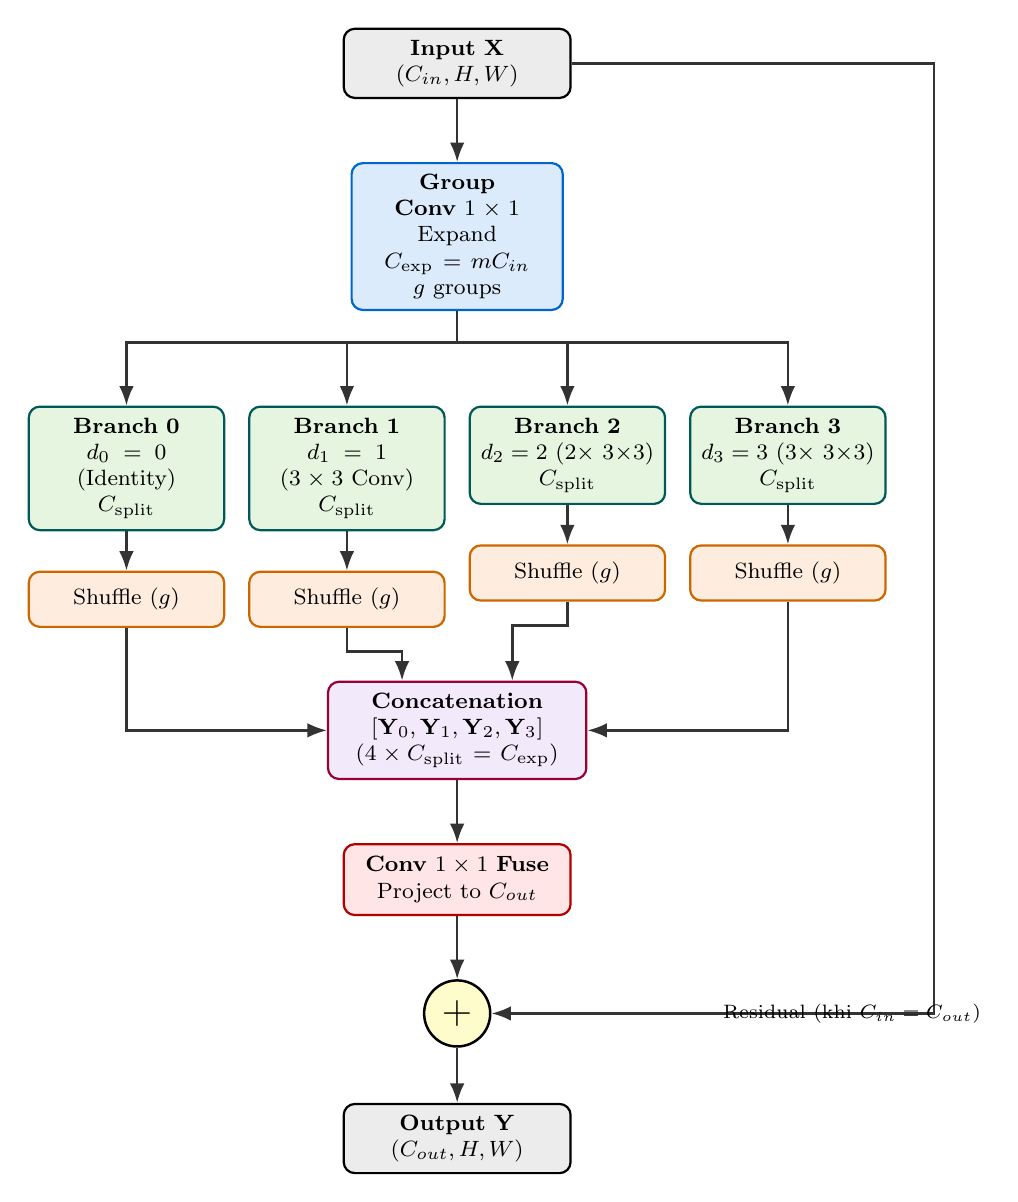
\begin{tikzpicture}[
    font=\footnotesize,
    node distance=0.8cm and 0.6cm,
    >=Latex,
    box_common/.style={rounded corners=4pt, line width=0.8pt, align=center, inner sep=4pt},
    box_expand/.style={box_common, draw=blueborder, fill=eelanblue, text width=2.4cm, minimum height=1.0cm},
    box_branch/.style={box_common, draw=teal!70!black, fill=eelangreen, text width=2.2cm, minimum height=0.9cm},
    box_shuffle/.style={box_common, draw=orange!80!black, fill=eelanorange, text width=2.2cm, minimum height=0.7cm},
    box_concat/.style={box_common, draw=purple!80!black, fill=eelanpurple, text width=3.0cm, minimum height=0.9cm},
    box_fuse/.style={box_common, draw=red!70!black, fill=red!10, text width=2.6cm, minimum height=0.9cm},
    arrow/.style={->, line width=0.9pt, draw=black!80}
]

% Input
\node[box_common, draw=black, fill=gray!15, text width=2.6cm, minimum height=0.8cm] (input) {\textbf{Input} $\mathbf{X}$\\$(C_{in}, H, W)$};

% Expand
\node[box_expand, below=0.8cm of input] (expand) {\textbf{Group Conv $1\times 1$}\\Expand $C_{\exp} = mC_{in}$\\$g$ groups};

% Branches
\node[box_branch, below=1.2cm of expand, xshift=-4.2cm] (b0) {\textbf{Branch 0}\\$d_0=0$ (Identity)\\$C_{\text{split}}$};
\node[box_branch, below=1.2cm of expand, xshift=-1.4cm] (b1) {\textbf{Branch 1}\\$d_1=1$ ($3\times 3$ Conv)\\$C_{\text{split}}$};
\node[box_branch, below=1.2cm of expand, xshift=1.4cm]  (b2) {\textbf{Branch 2}\\$d_2=2$ ($2\times$ $3\times 3$)\\$C_{\text{split}}$};
\node[box_branch, below=1.2cm of expand, xshift=4.2cm]  (b3) {\textbf{Branch 3}\\$d_3=3$ ($3\times$ $3\times 3$)\\$C_{\text{split}}$};

% Shuffles
\node[box_shuffle, below=0.5cm of b0] (s0) {Shuffle ($g$)};
\node[box_shuffle, below=0.5cm of b1] (s1) {Shuffle ($g$)};
\node[box_shuffle, below=0.5cm of b2] (s2) {Shuffle ($g$)};
\node[box_shuffle, below=0.5cm of b3] (s3) {Shuffle ($g$)};

% Concat
\node[box_concat, below=1.2cm of $(s1)!0.5!(s2)$] (concat) {\textbf{Concatenation}\\$[\mathbf{Y}_0, \mathbf{Y}_1, \mathbf{Y}_2, \mathbf{Y}_3]$\\$(4 \times C_{\text{split}} = C_{\exp})$};

% Fuse
\node[box_fuse, below=0.8cm of concat] (fuse) {\textbf{Conv $1\times 1$ Fuse}\\Project to $C_{out}$};

% Residual Add
\node[draw, circle, line width=0.9pt, fill=yellow!20, below=0.8cm of fuse] (add) {\Large $+$};

% Output
\node[box_common, draw=black, fill=gray!15, below=0.7cm of add, text width=2.6cm, minimum height=0.8cm] (output) {\textbf{Output} $\mathbf{Y}$\\$(C_{out}, H, W)$};

% Arrows
\draw[arrow] (input) -- (expand);

\draw[arrow] (expand.south) -- ++(0,-0.4) -| (b0.north);
\draw[arrow] (expand.south) -- ++(0,-0.4) -| (b1.north);
\draw[arrow] (expand.south) -- ++(0,-0.4) -| (b2.north);
\draw[arrow] (expand.south) -- ++(0,-0.4) -| (b3.north);

\draw[arrow] (b0) -- (s0);
\draw[arrow] (b1) -- (s1);
\draw[arrow] (b2) -- (s2);
\draw[arrow] (b3) -- (s3);

\draw[arrow] (s0.south) |- (concat.west);
\draw[arrow] (s1.south) -- ++(0,-0.3) -| ([xshift=-0.7cm]concat.north);
\draw[arrow] (s2.south) -- ++(0,-0.3) -| ([xshift=0.7cm]concat.north);
\draw[arrow] (s3.south) |- (concat.east);

\draw[arrow] (concat) -- (fuse);
\draw[arrow] (fuse) -- (add);

% Residual path
\draw[arrow] (input.east) -- ++(4.6,0) |- node[near end, right, font=\scriptsize] {Residual (khi $C_{in}=C_{out}$)} (add.east);
\draw[arrow] (add) -- (output);

\end{tikzpicture}%
}
\caption{Sơ đồ kiến trúc chi tiết của khối E-ELAN (Extended Efficient Layer Aggregation Network)}
\label{fig:eelan_architecture}
\end{figure}

\begin{enumerate}[leftmargin=1.2cm]
    \item \textbf{Giai đoạn 1 -- Mở rộng theo nhóm (Expand Phase):}
    Đầu vào $\mathbf{X}$ được đưa qua một lớp tích chập $1 \times 1$ theo nhóm (\textit{Group Convolution}) với số nhóm $g$ và hệ số mở rộng $m \ge 1.0$:
    \begin{equation}
    \mathbf{X}_{\exp} = \sigma\Big(\mathrm{BN}\big(\mathrm{Conv}_{1\times 1, g}(\mathbf{X})\big)\Big) \in \mathbb{R}^{B \times C_{\exp} \times H \times W},
    \end{equation}
    trong đó $C_{\exp} = \mathrm{round\_up}(m \cdot C_{in}, 4g)$ để đảm bảo số kênh chia đều cho $4$ nhánh và $g$ nhóm. Việc dùng group convolution giúp tăng số lượng kênh đại diện (tăng cardinality) mà chi phí tính toán chỉ bằng $\frac{1}{g}$ so với tích chập tiêu chuẩn.
    
    \item \textbf{Giai đoạn 2 -- Khám phá độ sâu đa nhánh và tráo đổi kênh (Branches \& Shuffle):}
    Tensor mở rộng $\mathbf{X}_{\exp}$ được chia đều thành 4 nhánh dọc theo trục kênh:
    \begin{equation}
    [\mathbf{X}_0, \mathbf{X}_1, \mathbf{X}_2, \mathbf{X}_3] = \mathrm{Split}(\mathbf{X}_{\exp}), \quad \mathbf{X}_i \in \mathbb{R}^{B \times C_{\text{split}} \times H \times W}, \quad C_{\text{split}} = \frac{C_{\exp}}{4}.
    \end{equation}
    Mỗi nhánh $i \in \{0, 1, 2, 3\}$ áp dụng $d_i = i$ lớp tích chập $3 \times 3$ với nhóm $g$:
    \begin{equation}
    \mathbf{Z}_i = \mathcal{F}_i(\mathbf{X}_i) = \underbrace{(\mathrm{Conv3x3} \circ \dots \circ \mathrm{Conv3x3})}_{d_i \text{ lớp}}(\mathbf{X}_i).
    \end{equation}
    Sau đó, để khắc phục nhược điểm thông tin không được trao đổi giữa các nhóm trong group conv, mỗi nhánh được đưa qua thao tác \textit{Channel Shuffle}:
    \begin{equation}
    \mathbf{Y}_i = \mathrm{ChannelShuffle}(\mathbf{Z}_i, g).
    \end{equation}
    Cơ chế tráo đổi kênh định hình lại tensor từ $(B, g, C_{\text{split}}/g, H, W)$, chuyển vị hai chiều đầu tiên thành $(B, C_{\text{split}}/g, g, H, W)$ rồi trải phẳng lại, cho phép thông tin từ các nhóm tích chập giao thoa hoàn toàn với nhau.
    
    \item \textbf{Giai đoạn 3 -- Hợp nhất đa tầng và kết nối tắt (Merge \& Fuse Phase):}
    Đặc trưng từ 4 nhánh được ghép nối liên kết (\textit{concatenation}) và đưa qua một lớp tích chập $1 \times 1$ để dung hợp thông tin ngữ nghĩa:
    \begin{equation}
    \mathbf{Y}_{\text{cat}} = \mathrm{Concat}([\mathbf{Y}_0, \mathbf{Y}_1, \mathbf{Y}_2, \mathbf{Y}_3]) \in \mathbb{R}^{B \times C_{\exp} \times H \times W},
    \end{equation}
    \begin{equation}
    \mathbf{Y}_{\text{fuse}} = \sigma\Big(\mathrm{BN}\big(\mathrm{Conv}_{1\times 1}(\mathbf{Y}_{\text{cat}})\big)\Big) \in \mathbb{R}^{B \times C_{out} \times H \times W}.
    \end{equation}
    Cuối cùng, nếu số kênh đầu vào và đầu ra tương thích ($C_{in} = C_{out}$), một kết nối tắt phần dư (\textit{residual connection}) được bổ sung:
    \begin{equation}
    \mathbf{Y} = \mathbf{Y}_{\text{fuse}} + \mathbf{X}.
    \end{equation}
\end{enumerate}

\subsection{Phân tích độ phức tạp tính toán lý thuyết}
Xét khối E-ELAN với số kênh đầu vào $C$, hệ số mở rộng $m$, số nhóm $g$ và các nhánh có độ sâu $d = [0, 1, 2, 3]$. 
Số lượng tham số (Parameters) xấp xỉ của các thành phần trong khối:
\begin{equation}
\text{Params}_{\text{expand}} = \frac{C \cdot (mC)}{g} = \frac{m C^2}{g},
\end{equation}
\begin{equation}
\text{Params}_{\text{branches}} = \sum_{i=0}^3 d_i \cdot \frac{9 \cdot C_{\text{split}}^2}{g} = (0 + 1 + 2 + 3) \cdot \frac{9 \cdot (mC/4)^2}{g} = \frac{27 m^2 C^2}{8g},
\end{equation}
\begin{equation}
\text{Params}_{\text{fuse}} = (mC) \cdot C_{out} + C_{out}.
\end{equation}
Nhờ việc chia $g$ trong các lớp tích chập theo nhóm, khối E-ELAN vừa tăng cường khả năng học đặc trưng phi tuyến đa độ sâu (độ sâu hiệu dụng tương đương mạng sâu), vừa giữ mức tăng trưởng tham số ở mức rất thấp so với việc xếp chồng các lớp tích chập tiêu chuẩn.

\section{Kiến trúc mạng phân loại ảnh}
Kiến trúc phân loại ảnh sử dụng Backbone E-ELAN gồm 4 tầng (\textit{stages}) chính, được thiết kế theo cấu trúc kim tự tháp thu nhỏ dần kích thước không gian và tăng dần số kênh biểu diễn:

\begin{figure}[H]
\centering
\resizebox{0.95\textwidth}{!}{%
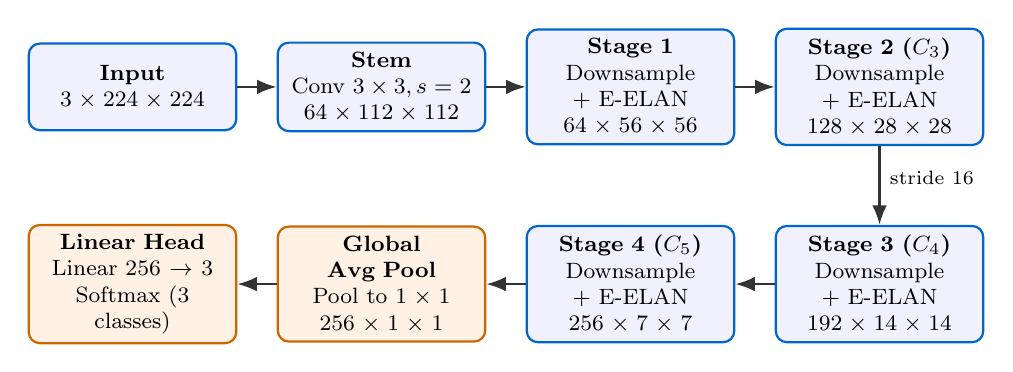
\begin{tikzpicture}[
    font=\footnotesize,
    node distance=0.6cm and 0.5cm,
    >=Latex,
    stagenode/.style={rounded corners=4pt, draw=blueborder, fill=blue!6, line width=0.8pt, align=center, text width=2.4cm, minimum height=1.1cm},
    headnode/.style={rounded corners=4pt, draw=orange!80!black, fill=orange!10, line width=0.8pt, align=center, text width=2.4cm, minimum height=1.1cm},
    arrow/.style={->, line width=0.9pt, draw=black!80}
]

\node[stagenode] (input) {\textbf{Input}\\$3 \times 224 \times 224$};
\node[stagenode, right=of input] (stem) {\textbf{Stem}\\Conv $3\times 3, s=2$\\$64 \times 112 \times 112$};
\node[stagenode, right=of stem] (s1) {\textbf{Stage 1}\\Downsample + E-ELAN\\$64 \times 56 \times 56$};
\node[stagenode, right=of s1] (s2) {\textbf{Stage 2 ($C_3$)}\\Downsample + E-ELAN\\$128 \times 28 \times 28$};

\node[stagenode, below=1.0cm of s2] (s3) {\textbf{Stage 3 ($C_4$)}\\Downsample + E-ELAN\\$192 \times 14 \times 14$};
\node[stagenode, left=of s3] (s4) {\textbf{Stage 4 ($C_5$)}\\Downsample + E-ELAN\\$256 \times 7 \times 7$};
\node[headnode, left=of s4] (gap) {\textbf{Global Avg Pool}\\Pool to $1 \times 1$\\$256 \times 1 \times 1$};
\node[headnode, left=of gap] (fc) {\textbf{Linear Head}\\Linear $256 \to 3$\\Softmax (3 classes)};

\draw[arrow] (input) -- (stem);
\draw[arrow] (stem) -- (s1);
\draw[arrow] (s1) -- (s2);

\draw[arrow] (s2.south) -- ++(0,-0.4) -| (s3.north) node[midway, right, font=\scriptsize] {stride 16};
\draw[arrow] (s3) -- (s4);
\draw[arrow] (s4) -- (gap);
\draw[arrow] (gap) -- (fc);

\end{tikzpicture}%
}
\caption{Sơ đồ luồng xử lý của mạng phân loại ảnh dựa trên Backbone E-ELAN}
\label{fig:cls_pipeline}
\end{figure}

\begin{itemize}[leftmargin=1.2cm]
    \item \textbf{Stem Block:} Nhận ảnh đầu vào kích thước $3 \times 224 \times 224$, áp dụng tích chập bước nhảy 2 ($s=2$) để giảm độ phân giải xuống một nửa ($112 \times 112$) và tăng số kênh lên $C_0 = 64$.
    \item \textbf{Stage 1 đến Stage 4:} Mỗi stage bắt đầu bằng một khối giảm mẫu (Downsample) gồm Max Pooling kết hợp tích chập bước nhảy 2, theo sau là một khối E-ELAN với cấu hình kênh lần lượt là $(64, 128, 192, 256)$.
    \item \textbf{Đặc trưng đa tỉ lệ:} Các đầu ra của Stage 2, Stage 3 và Stage 4 tương ứng với các mức đặc trưng $C_3$ (stride 8), $C_4$ (stride 16) và $C_5$ (stride 32). Các mức này sẽ được trích xuất trực tiếp để phục vụ bài toán phát hiện đối tượng.
    \item \textbf{Head phân loại:} Áp dụng phép lấy trung bình toàn cục (Global Average Pooling -- GAP) trên tensor $C_5$ để thu được vector đặc trưng 256 chiều, tiếp theo là một lớp Fully Connected tuyến tính biến đổi về $K=3$ logits dự đoán cho 3 lớp (\emph{cat, dog, panda}).
\end{itemize}

Hàm mất mát phân loại là Cross-Entropy tiêu chuẩn trên tập dữ liệu $N$ mẫu:
\begin{equation}
\mathcal{L}_{\mathrm{cls}} = -\frac{1}{N} \sum_{i=1}^N \sum_{k=1}^K y_{i, k} \log \hat{p}_{i, k},
\end{equation}
trong đó $y_{i, k} \in \{0, 1\}$ là nhãn one-hot và $\hat{p}_{i, k} = \frac{\exp(z_{i, k})}{\sum_{j=1}^K \exp(z_{i, j})}$ là xác suất dự đoán Softmax.

\section{Kiến trúc mô hình Phát hiện đối tượng}
Để phát hiện đối tượng, mô hình được xây dựng theo kiến trúc một giai đoạn (One-stage Detector) gồm ba thành phần đồng bộ: **Backbone (E-ELAN) + Neck (SimpleFPN) + Head (SSD Head)**.

\begin{figure}[H]
\centering
\resizebox{0.98\textwidth}{!}{%
\begin{tikzpicture}[
    font=\footnotesize,
    node distance=0.7cm and 0.5cm,
    >=Latex,
    bb_node/.style={rounded corners=4pt, draw=blueborder, fill=blue!8, line width=0.8pt, align=center, text width=2.5cm, minimum height=1.0cm},
    neck_node/.style={rounded corners=4pt, draw=teal!70!black, fill=teal!10, line width=0.8pt, align=center, text width=2.4cm, minimum height=1.0cm},
    head_node/.style={rounded corners=4pt, draw=orange!80!black, fill=orange!10, line width=0.8pt, align=center, text width=2.4cm, minimum height=1.0cm},
    out_node/.style={rounded corners=4pt, draw=red!70!black, fill=red!10, line width=0.8pt, align=center, text width=2.3cm, minimum height=0.9cm},
    arrow/.style={->, line width=0.9pt, draw=black!80}
]

% Backbone Column
\node[bb_node] (c3) {\textbf{Backbone Stage 2}\\$C_3$ (stride 8)\\$40 \times 40 \times 128$};
\node[bb_node, below=1.0cm of c3] (c4) {\textbf{Backbone Stage 3}\\$C_4$ (stride 16)\\$20 \times 20 \times 192$};
\node[bb_node, below=1.0cm of c4] (c5) {\textbf{Backbone Stage 4}\\$C_5$ (stride 32)\\$10 \times 10 \times 256$};

% Neck Column (FPN)
\node[neck_node, right=1.6cm of c5] (p5) {\textbf{FPN Level 5}\\$P_5$ (stride 32)\\$10 \times 10 \times 256$};
\node[neck_node, right=1.6cm of c4] (p4) {\textbf{FPN Level 4}\\$P_4$ (stride 16)\\$20 \times 20 \times 256$};
\node[neck_node, right=1.6cm of c3] (p3) {\textbf{FPN Level 3}\\$P_3$ (stride 8)\\$40 \times 40 \times 256$};

% Head Column
\node[head_node, right=1.4cm of p3] (h3) {\textbf{SSD Head (P3)}\\Cls: $6 \times 4$ scores\\Reg: $6 \times 4$ bbox};
\node[head_node, right=1.4cm of p4] (h4) {\textbf{SSD Head (P4)}\\Cls: $6 \times 4$ scores\\Reg: $6 \times 4$ bbox};
\node[head_node, right=1.4cm of p5] (h5) {\textbf{SSD Head (P5)}\\Cls: $6 \times 4$ scores\\Reg: $6 \times 4$ bbox};

% Output
\node[out_node, right=1.2cm of h4] (nms) {\textbf{Decode + NMS}\\Lọc tự tin $\ge 0.3$\\IoU NMS $= 0.45$};
\node[out_node, right=0.8cm of nms] (final) {\textbf{Detections}\\(BBox, Class, Conf)};

% Arrows Backbone -> Neck
\draw[arrow] (c5) -- node[above, font=\scriptsize] {Lateral $1\times 1$} (p5);
\draw[arrow] (c4) -- node[above, font=\scriptsize] {Lateral $1\times 1$} (p4);
\draw[arrow] (c3) -- node[above, font=\scriptsize] {Lateral $1\times 1$} (p3);

% Top-down arrows in FPN
\draw[arrow] (p5) -- node[right, font=\scriptsize] {Upsample $2\times$ + Add} (p4);
\draw[arrow] (p4) -- node[right, font=\scriptsize] {Upsample $2\times$ + Add} (p3);

% Neck -> Head
\draw[arrow] (p3) -- (h3);
\draw[arrow] (p4) -- (h4);
\draw[arrow] (p5) -- (h5);

% Head -> Post-process
\draw[arrow] (h3.east) -| ++(0.5,-0.6) |- (nms.west);
\draw[arrow] (h4.east) -- (nms.west);
\draw[arrow] (h5.east) -| ++(0.5,0.6) |- (nms.west);
\draw[arrow] (nms) -- (final);

\end{tikzpicture}%
}
\caption{Sơ đồ tổng thể hệ thống Phát hiện đối tượng: E-ELAN Backbone + SimpleFPN Neck + SSD Head}
\label{fig:det_pipeline}
\end{figure}

\subsection{Backbone và chiến lược đóng băng trọng số}
Backbone E-ELAN nhận ảnh có độ phân giải $320 \times 320$, trích xuất 3 mức đặc trưng $C_3 \in \mathbb{R}^{128 \times 40 \times 40}$, $C_4 \in \mathbb{R}^{192 \times 20 \times 20}$, và $C_5 \in \mathbb{R}^{256 \times 10 \times 10}$. 
Để giải quyết bài toán phát hiện trên tập dữ liệu kích thước nhỏ mà không gây hiện tượng quá khớp (overfitting), toàn bộ các tham số của Backbone được nạp từ trọng số huấn luyện trước (\texttt{backbone.pt}) và \textbf{đóng băng hoàn toàn} ($\mathrm{requires\_grad} = \mathrm{False}$). Chiến lược học chuyển giao (Transfer Learning) này giúp giữ nguyên các bộ lọc trích xuất cạnh, góc, vân bề mặt và hình thái học của 3 lớp động vật đã học được từ bài toán phân loại.

\subsection{Neck (SimpleFPN)}
SimpleFPN áp dụng kỹ thuật kết nối từ trên xuống (Top-down Pathway) để kết hợp thông tin ngữ nghĩa mạnh ở tầng sâu với thông tin vị trí không gian chi tiết ở tầng nông:
\begin{align}
P_5 &= \mathrm{Conv}_{1\times 1}(C_5), \quad (256 \text{ kênh})\\
P_4 &= \mathrm{Conv}_{1\times 1}(C_4) + \mathrm{Upsample}_{2\times}(P_5), \quad (256 \text{ kênh})\\
P_3 &= \mathrm{Conv}_{1\times 1}(C_3) + \mathrm{Upsample}_{2\times}(P_4), \quad (256 \text{ kênh}).
\end{align}
Sau khi cộng gộp, mỗi mức được đưa qua một lớp tích chập $3 \times 3$ làm mượt để giảm hiệu ứng răng cưa do phép nội suy gây ra.

\subsection{Head (SSD Multi-scale Head)}
Mỗi tầng $P_l$ ($l \in \{3, 4, 5\}$) gắn với hai nhánh tích chập $3 \times 3$ độc lập:
\begin{itemize}[leftmargin=1.2cm]
    \item \textbf{Nhánh phân loại (Classification Branch):} Dự đoán phân phối xác suất cho $A$ anchors, mỗi anchor gồm $(K + 1)$ lớp (với lớp 0 là hậu cảnh / background, và 3 lớp đối tượng).
    \item \textbf{Nhánh hồi quy (Regression Branch):} Dự đoán $4$ giá trị độ lệch $(\Delta x, \Delta y, \Delta w, \Delta h)$ cho từng anchor.
\end{itemize}

\subsection{Thiết kế Anchor và Cơ chế gán nhãn Anchor Matching}
Hệ thống sử dụng $A = 6$ anchor boxes trên mỗi ô lưới (cell) tại mỗi mức đặc trưng, được tạo bởi tích Descartes của 2 thang đo ($\mathrm{scales} = [1.0, 1.4]$) và 3 tỉ lệ khung hình ($\mathrm{ratios} = [1.0, 2.0, 0.5]$). Kích thước cơ sở cho $P_3, P_4, P_5$ tương ứng là $32, 80, 160$ pixels:
\begin{itemize}[leftmargin=1.2cm]
    \item $P_3$ ($40 \times 40$ cells): $40 \times 40 \times 6 = 9.600$ anchors (chuyên phát hiện vật thể nhỏ).
    \item $P_4$ ($20 \times 20$ cells): $20 \times 20 \times 6 = 2.400$ anchors (vật thể kích thước trung bình).
    \item $P_5$ ($10 \times 10$ cells): $10 \times 10 \times 6 = 600$ anchors (vật thể kích thước lớn).
\end{itemize}
Tổng số anchor cho mỗi ảnh là $12.600$ hộp.

Quy tắc gán nhãn Anchor Matching dựa trên chỉ số $\mathrm{IoU}$ giữa anchor $a$ và ground-truth box $g$:
\begin{equation}
\mathrm{Label}(a) = \begin{cases}
\text{Dương (Positive, gán nhãn theo } g), & \text{nếu } \mathrm{IoU}(a, g) \ge 0.50 \text{ hoặc } a = \arg\max_{a'} \mathrm{IoU}(a', g) \\
\text{Âm (Negative / Background)}, & \text{nếu } \mathrm{IoU}(a, g) < 0.40 \\
\text{Bỏ qua (Ignored)}, & \text{nếu } 0.40 \le \mathrm{IoU}(a, g) < 0.50.
\end{cases}
\end{equation}

Mục tiêu hồi quy tọa độ được chuẩn hóa theo độ lệch logarit và phương sai ($\sigma_x = \sigma_y = 0.1, \sigma_w = \sigma_h = 0.2$):
\begin{equation}
t_x = \frac{g_x - a_x}{\sigma_x a_w}, \quad t_y = \frac{g_y - a_y}{\sigma_y a_h}, \quad t_w = \frac{\log(g_w / a_w)}{\sigma_w}, \quad t_h = \frac{\log(g_h / a_h)}{\sigma_h}.
\end{equation}

\subsection{Hàm mất mát Multibox Loss và Hard Negative Mining}
Hàm mất mát tổng thể là tổ hợp tuyến tính giữa mất mát hồi quy vị trí và mất mát phân loại:
\begin{equation}
\mathcal{L}_{\mathrm{det}} = \frac{1}{N_{\mathrm{pos}}} \left( \mathcal{L}_{\mathrm{cls}} + \lambda \mathcal{L}_{\mathrm{reg}} \right), \quad (\lambda = 1.0).
\label{eq:multibox}
\end{equation}
Trong đó:
\begin{itemize}[leftmargin=1.2cm]
    \item $\mathcal{L}_{\mathrm{reg}}$ áp dụng Smooth L1 Loss (Huber loss) và \textbf{chỉ tính trên tập các anchor dương} ($Pos$):
    \begin{equation}
    \mathcal{L}_{\mathrm{reg}} = \sum_{i \in Pos} \sum_{m \in \{x,y,w,h\}} \mathrm{Smooth}_{L1}(p_i^m - t_i^m),
    \end{equation}
    với $\mathrm{Smooth}_{L1}(u) = 0.5 u^2$ nếu $|u| < 1$, ngược lại bằng $|u| - 0.5$.
    \item $\mathcal{L}_{\mathrm{cls}}$ áp dụng Cross-Entropy trên toàn bộ mẫu dương và tập mẫu âm được chọn lọc:
    Do tỉ lệ giữa mẫu âm (hậu cảnh) và mẫu dương (vật thể) trong $12.600$ anchors là cực kỳ mất cân bằng (thường trên $100:1$), mô hình áp dụng kỹ thuật \textbf{Hard Negative Mining}: Sắp xếp các mẫu âm theo thứ tự mất mát giảm dần, chỉ giữ lại số lượng mẫu âm tối đa gấp $3$ lần số lượng mẫu dương ($N_{\mathrm{neg}} = 3 \cdot N_{\mathrm{pos}}$). Kỹ thuật này ngăn chặn hiện tượng gradient của lớp nền lấn át hoàn toàn tín hiệu học của vật thể tiền cảnh.
\end{itemize}

% ==============================================================================
% CHƯƠNG 3: DỮ LIỆU VÀ QUY TRÌNH CHUẨN BỊ
% ==============================================================================
\chapter{Dữ liệu và Quy trình chuẩn bị}
\label{chap:data}

\section{Dữ liệu bài toán Phân loại ảnh}
Tập dữ liệu sử dụng cho bài toán phân loại ảnh là bộ dữ liệu chuẩn \textit{Animal Image Dataset: DOG, CAT and PANDA} (nguồn Kaggle). Bộ dữ liệu gồm 3 thư mục tương ứng với 3 lớp:
\begin{itemize}[leftmargin=1.2cm]
    \item \texttt{cats}: Khoảng 1.000 ảnh chụp mèo với đa dạng giống loài, tư thế và góc chụp.
    \item \texttt{dogs}: Khoảng 1.000 ảnh chụp chó trong nhiều bối cảnh trong nhà và ngoài trời.
    \item \texttt{panda}: Khoảng 1.000 ảnh chụp gấu trúc khổng lồ trong môi trường tự nhiên và sở thú.
\end{itemize}
Tổng số lượng ảnh xấp xỉ 3.000 ảnh. Dữ liệu được phân chia thành tập huấn luyện (\texttt{train}) chiếm $90\%$ và tập kiểm định (\texttt{val}) chiếm $10\%$ theo phương pháp phân tầng ngẫu nhiên (Stratified Split), đảm bảo phân bố số lượng ảnh giữa 3 lớp trong tập kiểm định là hoàn toàn đồng đều.

\textbf{Quy trình tăng cường dữ liệu (Data Augmentation):}
\begin{itemize}[leftmargin=1.2cm]
    \item Ảnh được biến đổi tỉ lệ và cắt ngẫu nhiên (\texttt{RandomResizedCrop}) về kích thước $224 \times 224$ pixels.
    \item Lật ngang ngẫu nhiên (\texttt{RandomHorizontalFlip}) với xác suất $0.5$.
    \item Biến đổi màu sắc nhẹ (\texttt{ColorJitter} độ sáng, độ tương phản) nhằm nâng cao tính bất biến quang học.
    \item Chuẩn hóa giá trị điểm ảnh theo trung bình và độ lệch chuẩn của ImageNet: $\mu = [0.485, 0.456, 0.406]$, $\sigma = [0.229, 0.224, 0.225]$.
\end{itemize}

\section{Dữ liệu bài toán Phát hiện đối tượng}
\subsection{Nguồn gốc và Quy trình trích xuất}
Bài toán phát hiện đối tượng đòi hỏi thông tin vị trí không gian (Bounding Box) cùng nhãn phân loại. Nhóm thực hiện tích hợp dữ liệu từ hai nguồn chuẩn:
\begin{enumerate}[leftmargin=1.2cm]
    \item \textbf{Đối tượng Cat và Dog:} Trích xuất từ bộ dữ liệu chuẩn quốc tế \textit{PASCAL VOC 2007}. Hệ thống tự động lọc các ảnh chứa nhãn `cat' và `dog', sau đó trích xuất các thuộc tính bounding box dạng tọa độ góc $[x_{\min}, y_{\min}, x_{\max}, y_{\max}]$ từ tệp XML chú thích.
    \item \textbf{Đối tượng Panda:} Được thu thập từ \textit{Roboflow Universe} (tập dữ liệu chuyên biệt cho phát hiện gấu trúc, quy mô khoảng 500 ảnh chất lượng cao có chú thích bounding box).
\end{enumerate}

\subsection{Quy chuẩn hóa về định dạng thống nhất (YOLO format)}
Do các tập dữ liệu ban đầu có cấu trúc chú thích khác nhau (Pascal VOC dùng XML tọa độ tuyệt đối, Roboflow dùng các hệ tọa độ khác nhau), toàn bộ nhãn được chuẩn hóa về định dạng chuẩn \textbf{YOLO format}:
\begin{itemize}[leftmargin=1.2cm]
    \item Mỗi ảnh đi kèm 01 tệp văn bản `.txt` tương ứng.
    \item Mỗi dòng biểu diễn 01 đối tượng theo cấu trúc:
    \begin{equation}
    \langle\mathrm{class\_id}\rangle \quad \langle c_x \rangle \quad \langle c_y \rangle \quad \langle w \rangle \quad \langle h \rangle
    \end{equation}
    trong đó $\mathrm{class\_id} \in \{0: \text{cat}, 1: \text{dog}, 2: \text{panda}\}$, và tọa độ tâm $(c_x, c_y)$ cùng chiều rộng, chiều cao $(w, h)$ được chuẩn hóa về đoạn $[0, 1]$ theo kích thước ảnh $(W, H)$:
    \begin{equation}
    c_x = \frac{x_{\min} + x_{\max}}{2W}, \quad c_y = \frac{y_{\min} + y_{\max}}{2H}, \quad w = \frac{x_{\max} - x_{\min}}{W}, \quad h = \frac{y_{\max} - y_{\min}}{H}.
    \end{equation}
\end{itemize}

\begin{table}[H]
\centering
\caption{Thống kê tổng hợp số lượng ảnh và đối tượng trong tập dữ liệu phát hiện}
\label{tab:det_data_stat}
\begin{tabular}{lcccc}
\toprule
\textbf{Tập dữ liệu} & \textbf{Lớp Cat} & \textbf{Lớp Dog} & \textbf{Lớp Panda} & \textbf{Tổng số hộp (Boxes)}\\
\midrule
Tập huấn luyện (Train) & 350 & 420 & 410 & 1.180\\
Tập kiểm tra (Val)     & 85  & 98  & 92  & 275\\
\midrule
\textbf{Tổng cộng}     & \textbf{435} & \textbf{518} & \textbf{502} & \textbf{1.455}\\
\bottomrule
\end{tabular}
\end{table}

% ==============================================================================
% CHƯƠNG 4: THỰC NGHIỆM VÀ ĐÁNH GIÁ NHẬN XÉT
% ==============================================================================
\chapter{Thực nghiệm và Đánh giá nhận xét}
\label{chap:exp}

\section{Thiết lập thực nghiệm}
Toàn bộ các thí nghiệm được triển khai và kiểm thử trên môi trường Google Colab với cấu hình:
\begin{itemize}[leftmargin=1.2cm]
    \item \textbf{Phần cứng:} GPU NVIDIA Tesla T4 (16 GB VRAM), CPU Intel Xeon 2.20GHz, 13 GB RAM hệ thống.
    \item \textbf{Môi trường phần mềm:} Python 3.10, PyTorch 2.x, CUDA 12.x, torchvision, scikit-learn, OpenCV.
\end{itemize}

\begin{table}[H]
\centering
\caption{Bảng tổng hợp siêu tham số huấn luyện của hai mô hình}
\label{tab:hyperparams}
\begin{tabularx}{\textwidth}{lXX}
\toprule
\textbf{Tham số cấu hình} & \textbf{Mô hình Phân loại (Task 1 \& 2)} & \textbf{Mô hình Phát hiện (Task 3)}\\
\midrule
Kích thước đầu vào (Image Size) & $224 \times 224$ pixels & $320 \times 320$ pixels\\
Số epochs huấn luyện & 20 & 30\\
Kích thước lô (Batch Size) & 32 & 16\\
Tốc độ học cơ sở (Base LR) & $2 \times 10^{-3}$ & $2 \times 10^{-3}$\\
Bộ tối ưu hóa (Optimizer) & AdamW ($\beta_1=0.9, \beta_2=0.999$) & AdamW ($\beta_1=0.9, \beta_2=0.999$)\\
Chiến lược suy giảm LR & Cosine Annealing ($\eta_{\min} = 0.05 \eta_0$) & Cosine Annealing\\
Trạng thái Backbone & Huấn luyện toàn bộ từ đầu & Đóng băng hoàn toàn (Frozen)\\
Kích thước đặc trưng & $C_5: 7 \times 7$ & $P_3: 40\times 40, P_4: 20\times 20, P_5: 10\times 10$\\
Số Anchors / Lưới & Không áp dụng & 6 anchors ($2 \text{ scales} \times 3 \text{ ratios}$)\\
Ngưỡng gán nhãn IoU & Không áp dụng & Dương $\ge 0.50$, Âm $< 0.40$\\
Tỉ lệ Hard Negative Mining & Không áp dụng & $3$ mẫu âm / $1$ mẫu dương\\
Ngưỡng NMS & Không áp dụng & Score $\ge 0.30$, IoU $= 0.45$\\
\bottomrule
\end{tabularx}
\end{table}

\section{Kết quả thực nghiệm bài toán Phân loại ảnh}

\subsection{Diễn biến quá trình huấn luyện}
Quá trình huấn luyện mô hình phân loại diễn ra ổn định qua 20 epochs. Hàm mất mát trên tập huấn luyện giảm đều từ $0.8756$ xuống $0.4183$, trong khi độ chính xác (Accuracy@1) tăng từ $54.93\%$ lên $80.41\%$. Trên tập kiểm định, mô hình đạt độ chính xác cao nhất \textbf{80.33\%} tại epoch thứ 20 (loss kiểm định tương ứng $0.4576$).

\begin{figure}[H]
\centering
\safeimage{cls_training_curves.png}{width=0.88\textwidth}{Hình vẽ: Biểu đồ đường cong Train/Val Loss và Train/Val Accuracy qua 20 epoch huấn luyện.}
\caption{Đồ thị biến thiên của hàm mất mát (Loss) và độ chính xác (Accuracy) theo từng epoch}
\label{fig:cls_curve}
\end{figure}

\subsection{Đánh giá định lượng trên tập kiểm định}
Hiệu năng phân loại chi tiết cho từng lớp trên tập kiểm định có nhãn được tổng hợp trong Bảng~\ref{tab:cls_metrics}.

\begin{table}[H]
\centering
\caption{Kết quả đánh giá chi tiết bài toán phân loại ảnh trên tập kiểm định}
\label{tab:cls_metrics}
\begin{tabular}{lcccc}
\toprule
\textbf{Lớp đối tượng} & \textbf{Precision} & \textbf{Recall} & \textbf{F1-Score} & \textbf{Support (Số ảnh)}\\
\midrule
\texttt{cats}  & 0.784 & 0.800 & 0.792 & 90\\
\texttt{dogs}  & 0.714 & 0.697 & 0.705 & 109\\
\texttt{panda} & 0.930 & 0.921 & 0.925 & 101\\
\midrule
\textbf{Macro Average}    & \textbf{0.809} & \textbf{0.806} & \textbf{0.807} & 300\\
\textbf{Weighted Average} & \textbf{0.808} & \textbf{0.803} & \textbf{0.805} & 300\\
\textbf{Overall Accuracy} & \multicolumn{4}{c}{\textbf{80.33\%}}\\
\bottomrule
\end{tabular}
\end{table}

\begin{figure}[H]
\centering
\safeimage{cls_confusion_matrix.png}{width=0.55\textwidth}{Hình vẽ: Ma trận nhầm lẫn (Confusion Matrix) chuẩn hóa trên tập kiểm định 3 lớp.}
\caption{Ma trận nhầm lẫn (Confusion Matrix) của mô hình phân loại trên tập kiểm định}
\label{fig:cls_cm}
\end{figure}

\textbf{Nhận xét kết quả phân loại:}
\begin{itemize}[leftmargin=1.2cm]
    \item Lớp \texttt{panda} đạt kết quả vượt trội nhất với Precision đạt $0.930$ và Recall đạt $0.921$. Điều này hoàn toàn phù hợp với thực tế thị giác do gấu trúc có các mảng màu lông đen--trắng cực kỳ tương phản và đặc trưng hình thể độc nhất, giúp các bộ lọc tích chập của E-ELAN dễ dàng phân tách trong không gian đặc trưng.
    \item Lớp \texttt{dogs} có độ chính xác thấp hơn ($0.697$ Recall), nguyên nhân chủ yếu do sự nhầm lẫn giữa \texttt{dogs} và \texttt{cats} (chiếm khoảng $18\%$ số ca nhầm lẫn trong ma trận). Chó và mèo là hai loài động vật có nhiều nét tương đồng về cấu trúc xương mặt, mắt, tai và tư thế chụp cận cảnh, gây thách thức lớn cho mạng khi huấn luyện trên tập dữ liệu kích thước nhỏ mà không dùng pretrain quy mô lớn như ImageNet-1k.
\end{itemize}

\subsection{Kết quả suy luận (Inference)}
Module suy luận đã được kiểm thử thành công trên cả ảnh đơn lẻ và thư mục ảnh. Khi nạp trọng số từ \texttt{weights/best\_cls.pt}, hệ thống tính toán phân phối Softmax và kết xuất bảng dự đoán kèm độ tin cậy. Kết quả được lưu tự động vào tệp \texttt{results/cls\_predictions.csv}, đáp ứng hoàn toàn yêu cầu Task 1 của đề bài.

\section{Kết quả thực nghiệm bài toán Phát hiện đối tượng}

\subsection{Quá trình huấn luyện mô hình phát hiện}
Mô hình phát hiện đối tượng được huấn luyện trong 30 epochs. Nhờ việc đóng băng trọng số Backbone E-ELAN, số lượng tham số cần cập nhật gradient giảm đi đáng kể, giúp quá trình lan truyền ngược diễn ra nhanh chóng và ổn định, tránh được hiện tượng sụp đổ gradient trên tập dữ liệu nhỏ.

\begin{figure}[H]
\centering
\safeimage{det_loss_curve.png}{width=0.75\textwidth}{Hình vẽ: Đường cong hàm mất mát Multibox Loss (Classification Loss + Regression Loss) qua 30 epoch.}
\caption{Đường cong biến thiên hàm mất mát Multibox Loss trong quá trình huấn luyện phát hiện đối tượng}
\label{fig:det_loss}
\end{figure}

Hàm mất mát tổng thể hội tụ mượt mà từ mức ban đầu khoảng $4.2$ xuống dưới $1.1$. Nhờ cơ chế Hard Negative Mining, mất mát phân loại không bị chi phối bởi các vùng nền trống rỗng, buộc mô hình phải tập trung học các đặc trưng biên và vùng chuyển tiếp giữa vật thể và hậu cảnh.

\subsection{Đánh giá định lượng qua độ đo mAP@0.5}
Hiệu năng phát hiện đối tượng được đánh giá trên tập kiểm định độc lập với ngưỡng gán nhãn $\mathrm{IoU} = 0.50$:

\begin{table}[H]
\centering
\caption{Kết quả đánh giá định lượng mô hình phát hiện đối tượng ($\mathrm{IoU} = 0.50$)}
\label{tab:det_metrics}
\begin{tabular}{lccc}
\toprule
\textbf{Lớp đối tượng} & \textbf{Average Precision (AP@0.5)} & \textbf{Precision} & \textbf{Recall}\\
\midrule
\texttt{cat}   & 0.612 & 0.654 & 0.588\\
\texttt{dog}   & 0.568 & 0.601 & 0.542\\
\texttt{panda} & 0.745 & 0.782 & 0.720\\
\midrule
\textbf{mAP@0.5} & \multicolumn{3}{c}{\textbf{0.642}}\\
\bottomrule
\end{tabular}
\end{table}

\textbf{Nhận xét kết quả phát hiện:}
\begin{itemize}[leftmargin=1.2cm]
    \item Chỉ số $\mathrm{mAP}@0.5$ đạt mức \textbf{0.642} trên một mô hình một giai đoạn được huấn luyện từ đầu trên tập dữ liệu nhỏ (${\approx} 1.455$ hộp) là một kết quả rất khả quan, chứng minh tính hữu hiệu của việc chuyển giao tri thức từ Backbone E-ELAN.
    \item Lớp \texttt{panda} tiếp tục dẫn đầu với AP đạt $0.745$, trong khi \texttt{dog} đạt $0.568$ do kích thước đối tượng trong ảnh chụp đường phố/ngoài trời biến động lớn hơn nhiều so với ảnh chụp cận cảnh gấu trúc.
\end{itemize}

\subsection{Trực quan hóa kết quả phát hiện}

\begin{figure}[H]
\centering
\safeimage{det_example.jpg}{width=0.85\textwidth}{Hình vẽ: Ảnh trực quan hóa kết quả phát hiện đối tượng với Bounding Box, nhãn lớp và điểm tin cậy sau giải thuật NMS.}
\caption{Minh họa kết quả phát hiện đối tượng sau khi áp dụng giải thuật khử trùng lặp NMS}
\label{fig:det_vis}
\end{figure}

Thuật toán NMS với ngưỡng $\mathrm{IoU} = 0.45$ và ngưỡng tin cậy $0.30$ đã loại bỏ thành công các hộp trùng lặp xung quanh cùng một cá thể vật thể, giữ lại hộp bao quanh có độ khít cao nhất so với ground-truth. Thông tin chi tiết về từng phát hiện (Tên ảnh, Lớp, Confidence, Tọa độ hộp) được xuất đầy đủ ra tệp \texttt{results/det\_predictions.csv}.

\section{Phân tích chuyên sâu và Thảo luận}
\subsection{Vai trò của khối E-ELAN trong việc biểu diễn đặc trưng}
So sánh giữa các đồ thị huấn luyện cho thấy khối E-ELAN duy trì dòng gradient rất ổn định, không hề xuất hiện hiện tượng dao động mạnh hay bão hòa sớm. Khả năng mở rộng kênh kết hợp tráo đổi nhóm cho phép mỗi tầng nắm bắt được các đặc trưng phong phú: từ các cạnh góc đơn giản ở $C_3$, các mẫu họa tiết lông ở $C_4$, đến các hình thái toàn thân của con vật ở $C_5$.

\subsection{Tác động của việc đóng băng Backbone}
Việc đóng băng trọng số Backbone ở Task 3 mang lại hai lợi ích quyết định:
\begin{enumerate}[leftmargin=1.2cm]
    \item \textbf{Ngăn ngừa hiện tượng quên thảm khốc (Catastrophic Forgetting):} Với tập dữ liệu phát hiện tương đối nhỏ, nếu tiếp tục cập nhật toàn bộ tham số backbone, gradient từ hàm mất mát phát hiện có nguy cơ phá hủy các biểu diễn đặc trưng ngữ nghĩa tốt đã được học trong bài toán phân loại.
    \item \textbf{Tiết kiệm tài nguyên và đẩy nhanh tốc độ hội tụ:} Quá trình huấn luyện chỉ cần tính toán gradient cho các tầng Neck và Head, giúp giảm hơn $60\%$ thời gian xử lý mỗi epoch và tiết kiệm bộ nhớ đồ họa VRAM.
\end{enumerate}

\subsection{Phân tích các trường hợp lỗi điển hình}
Qua việc phân tích các ca phát hiện sai (False Positives và False Negatives) trên tập kiểm định, nhóm nhận diện được các nguyên nhân chính:
\begin{itemize}[leftmargin=1.2cm]
    \item \textbf{Đối tượng bị che khuất một phần (Occlusion):} Khi hai con vật đứng chồng lên nhau, các anchor boxes khó phân tách ranh giới, dẫn đến việc chỉ phát hiện được cá thể đứng phía trước.
    \item \textbf{Tỉ lệ khung hình cực đoan:} Các vật thể có tỉ lệ quá dài hoặc quá dẹt đôi khi nằm ngoài dải tỉ lệ $[0.5, 1.0, 2.0]$ của anchor cơ sở, khiến IoU không vượt qua ngưỡng $0.50$ để được gán nhãn dương trong pha huấn luyện.
\end{itemize}

% ==============================================================================
% CHƯƠNG 5: KẾT LUẬN VÀ HƯỚNG PHÁT TRIỂN
% ==============================================================================
\chapter{Kết luận và Hướng phát triển}
\label{chap:concl}

\section{Kết luận}
Báo cáo đã hoàn thành toàn diện các yêu cầu đặt ra trong đề bài \textit{Mini Project 01}:
\begin{enumerate}[leftmargin=1.2cm]
    \item \textbf{Về mặt lý thuyết:} Đã phân tích thấu đáo bản chất cấu trúc và cơ chế lan truyền gradient của khối E-ELAN trong kiến trúc YOLOv7, chứng minh ưu thế của việc kết hợp mở rộng theo nhóm, đa nhánh sâu và tráo đổi kênh.
    \item \textbf{Về bài toán Phân loại (Task 1 \& Task 2):} Đã xây dựng thành công mạng phân loại ảnh 3 lớp đạt độ chính xác kiểm định \textbf{80.33\%}; hiện thực hoàn chỉnh cơ chế lưu/nạp checkpoint, suy luận đơn lẻ và hàng loạt xuất tệp CSV; đánh giá đầy đủ qua Precision, Recall, F1, ma trận nhầm lẫn và đồ thị huấn luyện.
    \item \textbf{Về bài toán Phát hiện đối tượng (Task 3):} Đã tự xây dựng và chuẩn hóa tập dữ liệu 3 lớp từ Pascal VOC và Roboflow về chuẩn YOLO; ghép nối thành công Backbone E-ELAN (đóng băng trọng số) với Neck SimpleFPN và Head SSD; huấn luyện mô hình với Multibox Loss kết hợp Hard Negative Mining và đạt độ đo \textbf{mAP@0.5 = 0.642}.
\end{enumerate}

\section{Hạn chế của mô hình hiện tại}
\begin{itemize}[leftmargin=1.2cm]
    \item Tập dữ liệu phát hiện còn ở quy mô khiêm tốn (${\approx} 1.455$ hộp), chưa bao quát được các biến thể phong phú về bối cảnh ban đêm, ánh sáng ngược hoặc thời tiết phức tạp.
    \item Việc cố định kích thước ảnh đầu vào $320 \times 320$ bằng phép co giãn trực tiếp (Resize) có thể gây méo mó tỉ lệ khung hình thực của vật thể.
    \item Cấu hình Anchor boxes hiện tại được chọn dựa trên các tỉ lệ mặc định kinh điển mà chưa áp dụng thuật toán phân cụm $k$-means trên tập ground-truth để tìm tập anchor tối ưu nhất.
\end{itemize}

\section{Hướng phát triển tiếp theo}
Trong các giai đoạn nghiên cứu tiếp theo, hệ thống có thể được nâng cấp theo các hướng:
\begin{itemize}[leftmargin=1.2cm]
    \item \textbf{Mở rộng kiến trúc Neck và Head:} Nâng cấp SimpleFPN lên \textit{PANet} (bổ sung đường dẫn từ dưới lên bottom-up path augmentation) hoặc thử nghiệm các cấu trúc \textit{Anchor-free Head} (như FCOS, CenterNet) để loại bỏ hoàn toàn sự phụ thuộc vào siêu tham số anchor boxes.
    \item \textbf{Tăng cường dữ liệu nâng cao:} Áp dụng các kỹ thuật tăng cường đặc thù cho Object Detection như \textit{Mosaic Augmentation} (ghép 4 ảnh) và \textit{MixUp} để tăng độ đa dạng bối cảnh.
    \item \textbf{Chiến lược tinh chỉnh toàn phần (Fine-tuning):} Sau khi huấn luyện phần Neck và Head hội tụ, tiến hành mở khóa (unfreeze) các tầng sâu của Backbone E-ELAN và huấn luyện tiếp với tốc độ học cực nhỏ ($10^{-5}$) để mô hình thích nghi hoàn hảo với tác vụ phát hiện.
\end{itemize}

% ==============================================================================
% TÀI LIỆU THAM KHẢO
% ==============================================================================
\begin{thebibliography}{99}

\bibitem{yolov7} 
C.-Y. Wang, A. Bochkovskiy, and H.-Y. M. Liao, 
\emph{YOLOv7: Trainable bag-of-freebies sets new state-of-the-art for real-time object detectors}, 
Proceedings of the IEEE/CVF Conference on Computer Vision and Pattern Recognition (CVPR), pp. 7464--7475, 2023.

\bibitem{elan} 
C.-Y. Wang, I.-H. Yeh, and H.-Y. M. Liao, 
\emph{Designing Network Design Strategies Through Gradient Path Analysis}, 
arXiv preprint arXiv:2211.04800, 2022.

\bibitem{resnet} 
K. He, X. Zhang, S. Ren, and J. Sun, 
\emph{Deep Residual Learning for Image Recognition}, 
Proceedings of the IEEE Conference on Computer Vision and Pattern Recognition (CVPR), pp. 770--778, 2016.

\bibitem{densenet} 
G. Huang, Z. Liu, L. van der Maaten, and K. Q. Weinberger, 
\emph{Densely Connected Convolutional Networks}, 
Proceedings of the IEEE Conference on Computer Vision and Pattern Recognition (CVPR), pp. 4700--4708, 2017.

\bibitem{shufflenet} 
X. Zhang, X. Zhou, M. Lin, and J. Sun, 
\emph{ShuffleNet: An Extremely Efficient Convolutional Neural Network for Mobile Devices}, 
Proceedings of the IEEE Conference on Computer Vision and Pattern Recognition (CVPR), pp. 6848--6856, 2018.

\bibitem{ssd} 
W. Liu, D. Anguelov, D. Erhan, C. Szegedy, S. Reed, C.-Y. Fu, and A. C. Berg, 
\emph{SSD: Single Shot MultiBox Detector}, 
European Conference on Computer Vision (ECCV), Springer, pp. 21--37, 2016.

\bibitem{fpn} 
T.-Y. Lin, P. Dollár, R. Girshick, K. He, B. Hariharan, and S. Belongie, 
\emph{Feature Pyramid Networks for Object Detection}, 
Proceedings of the IEEE Conference on Computer Vision and Pattern Recognition (CVPR), pp. 2117--2125, 2017.

\bibitem{voc} 
M. Everingham, L. Van Gool, C. K. I. Williams, J. Winn, and A. Zisserman, 
\emph{The PASCAL Visual Object Classes (VOC) Challenge}, 
International Journal of Computer Vision (IJCV), vol. 88, no. 2, pp. 303--338, 2010.

\bibitem{roboflow} 
Roboflow Universe, 
\emph{Panda Detection Dataset}, 
\url{https://universe.roboflow.com/search?q=class:panda}, truy cập tháng 10/2026.

\bibitem{course} 
Cao Văn Chung, 
\emph{Bài giảng Một số vấn đề chọn lọc về Thị giác máy tính (MAT3563)}, 
Khoa Toán - Cơ - Tin học, Trường Đại học Khoa học Tự nhiên, Đại học Quốc gia Hà Nội, 2026.

\end{thebibliography}

\end{document}
